% Usar el tipo de documento: Artículo científico.
\documentclass[12pt,a4paper]{article}

% Cargar mensajes en español.
\usepackage[spanish]{babel}

% Usar codificación utf-8 para acentos y otros.
\usepackage[utf8]{inputenc}


% Insertar porciones de código
\usepackage{listings}

% Comenzar párrafos con separación no indentación
\usepackage{parskip}

% Configuración para porciones de código
\lstset{
%	language=bash,
	basicstyle=\ttfamily\small,
%	numberstyle=\footnotesize,
%	numbers=left,
%	backgroundcolor=\color{gray!10},
%	frame=single,
	tabsize=4,
%	rulecolor=\color{black!30},
%	title=\lstname,
%	escapeinside={\%*}{*)},
	breaklines=true,
	breakatwhitespace=true,
%	framextopmargin=2pt,
%	framexbottommargin=2pt,
	extendedchars=false,
	inputencoding=utf8
}
% % path imagenes
\usepackage{graphicx}
\graphicspath{ {img/} }
%%%%%%%%%%%%%%%%%%%%%%%%%%%%%%%%%%%%%%%%%%%%%%%%%%%%%%%%%%%%%%%%%%%%%%%%%%%%%%%

% Propiedades
\title{Análisis de lenguajes programación orientados a niños.}

\author{Andrés Baamonde Lozano (andres.baamonde@udc.es)\\
	Rodrigo Arias Mallo (rodrigo.arias@udc.es)}

\begin{document}

\maketitle

%%%%%%%%%%%%%%%%%%%%%%%%%%%%%%%%%%%%%%%%%%%%%%%%%%%%%%%%%%%%%%%%%%%%%%%%%%%%%%%
\section{Lego Mindstorms EV3}
\subsection{Introducción}
   Mindstorms EV3 es un lenguaje de programación creado para los para interactuar con el kit Mindstorms EV3 de Lego. Esta diseñado para que Robots modulares que se construyen con piezas de lego por lo que son de coste "reducido".Estos robots utilizan piezas de la linea Technic con sensores y actuadores de bajo coste, con un módulo de control (brick) que tiene la potencia de un smartphone de gama baja.
  \subsection{Características del brick}
  \begin{itemize}
  \item Procesador ARM9 @300MHz.
  \item 16 MB Flash (Linux).
  \item 64 MB RAM.
  \item 4 puertos de entrada para sensores y 4 puertos de salida para actuadores.
  \item Ranura microSDHC (hasta 32 GB). Se puede arrancar un S.O. diferente al que trae de
  serie desde una tarjeta en esta ranura.
  \item Bluetooth.
  \item Soporta wifi (sin encriptación o con WPA2) conectando dongle NetGear WNA1100 en
  puerto USB.
  \item Se pueden conectar hasta 4 bricks en daisy chaining para ampliar el número de puertos
  para sensores y actuadores (el programa se ejecuta solo en uno de los bricks).
  \end{itemize}
  \subsection{Sofware de Programación}
  \subsubsection{De ejecución del brick}
    \begin{itemize}
    \item Mindstorms EV3(el que trataremos).
    \item RobotC for LEGO Mindstorms.
    \item MonoBrick(Alfa).
    \item LabVIEW(En desarrollo).
    \item BricxCC(En desarrollo).
    \item Python EV3(En desarrollo).
    \item LeJOS(Beta).
    \end{itemize}
  \subsubsection{De control remoto}
      \begin{itemize}
      \item Microsoft EV3 API.
      \item MonoBrick.
      \item RWTH Toolbox para Matlab(En desarrollo).
      \end{itemize}
\section{Mindstorms EV3}
\subsection{Características}
\subsubsection{Pros}
      \begin{itemize}
      \item Muy fácil construir comportamientos reactivos / programar autómatas.
      \item Curva de aprendizaje muy rápida para quien no haya programado antes en otro lenguaje.
      \item Fomenta la documentación de los programas.
      \item Ejecución paralela trivial.
      \item Herramienta de data logging muy sencilla de utilizar.
      \item Muy buena documentación disponible en su propio servidor web (http://localhost:58401).
      \end{itemize}
\subsubsection{Contras}
      \begin{itemize}
      \item Tedioso manejar estructuras de datos complejas.
      \item La programación es lenta si se compara con un lenguaje tradicional una vez que se domina éste.
      \item Programas medianos o grandes complicados de gestionar. Es necesario acostumbrarse a particionar todo en bloques propios.
      \item No hay simulador (aunque se puede acoplar al Robot Virtual Worlds).
      \end{itemize}
\subsection{El entorno de programación}
\subsubsection{Ventana}
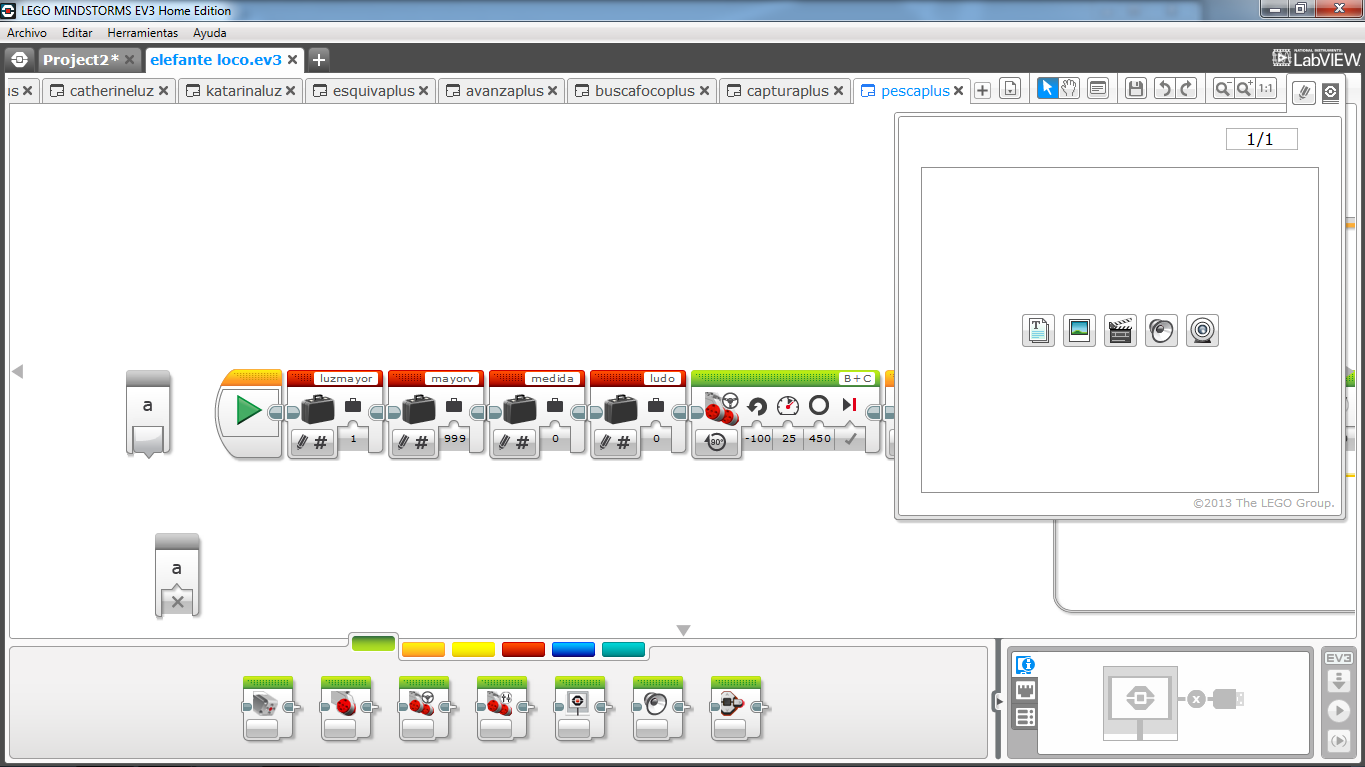
\includegraphics[scale=0.45]{Programa.PNG}
\subsubsection{Proyecto}
\includegraphics[scale=0.5]{image28.jpg}
\subsubsection{Página de hardware}
\section{Lenguaje de Programación}
\subsection{Introducción}
\subsection{Secuencias de Bloques}
\subsection{Secuencias Paralelas}
\subsection{Creación de bloques}
\subsection{Tipos de datos}
\subsection{Cables de datos}
\subsection{Variables y constantes}
\subsubsection{Variables}
\subsubsection{Constantes}
\subsection{Bloques predefinidos}
\subsection{Flujo de un programa}
\subsubsection{Iniciar}
\subsubsection{detener}
\subsection{E/S básica}
\end{document}
